
\section{Knowledge Modeling - Graph Databases}
The goal is to turn schema-less data into data with schema by exploiting the embedded schema information and identifying the structural regularities in a given database. 

\subsection{Graph Data Model}
The graph data model is used as it can generalize common data models (e.g. relational, XML, RDF, etc).
\subsubsection{Formal Definition} 
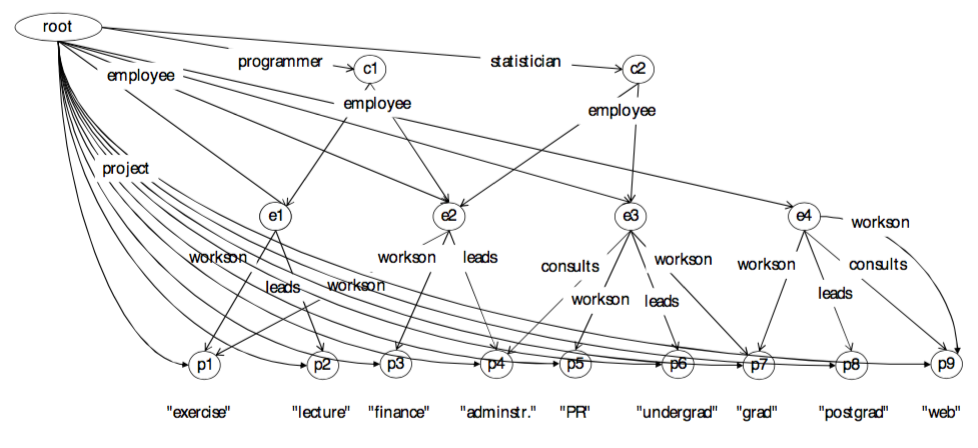
\includegraphics[width=\textwidth]{figures/data_graph.png}
\begin{itemize}
  \item Data graph: D = (V, E, R) is a labeled, rooted and directed graph 
  \item V is a set of nodes
  \item E $\subseteq$ V x L x V is a set of labeled edges, they determine the meaning of the data values stored in the leaves
  \item R $\subseteq$ V is a set of root nodes that have no incoming edges. All nodes in V are reachable from some root in R
  \item A $\subseteq$ V are the atomic nodes = set of leaf nodes storing typed data values
  \item C $\subseteq$ A x U x T is the data stored in D, where U is the domain of all data values and T are the data types
\end{itemize}

\subsubsection{Structural Properties}
We can enumerate the paths starting from the root to capture the structure of the data graph. A possible schema would be to use a \textbf{trie} enumerating those paths and labeling the leaf nodes with the data type that is found in the graph database. However, it contains many redundant structures so it would be better to combine different subgraphs into a common graph structure. 

\subsubsection{Simulation and Schema Graphs}
Simulation is used to provide a criterion to decide whether a schema graph S correctly captures the structure of a data graph D. A schema graph may use alternate labels or wildcards on edges. Condition: for every node d in D reached by a path p starting from the root there exists a corresponding node s in S reachable by the same path and the types of the leaf nodes are the same in case d is a leaf node. S simulates D is denoted as D $<$ S.

More formal definition of the simulation relationship among labelled graphs:
\begin{itemize}
  \item Given graphs G$_{1}$, G$_{2}$ and relation R $\subseteq$ V$_{1}$ x V$_{2}$, then R is a simulation if for all labels l $\in$ L and for all x$_{1}$, y$_{1}$ $\in$ V$_{1}$ and for all x$_{2}$ $\in$ V$_{2}$ it holds that if x$_{1}$ $\rightarrow$$_{l}$ y$_{1}$ and R(x$_{1}$, x$_{2}$) then there exists y$_{2}$ $\in$ V$_{2}$ such that R(y$_{1}$, y$_{2}$) and x$_{2}$ $\rightarrow$$_{l}$ y$_{2}$
  \item If it holds, G$_{2}$ simulates G$_{1}$ and we can write G$_{1}$ $<$ G$_{2}$
\end{itemize}

We have to extend the concept of simulation relationship for the graph data model:
\begin{itemize}
  \item A schema graph S is a schema for a data graph D if there exists a rooted, typed simulation of D using S (that may contain wildcards and alternate labels). We require that root and leaf nodes in the data graph are related to root and leaf nodes in the schema graph. 
  \item Rooted simulation: R(r$_{1}$, r$_{2}$) for the roots r$_{1}$ and r$_{2}$  
  \item Typed simulation: for all x, y if R(x, y) and y is an atomic type then x must be an atomic node with content of that type
  \item For wildcards and alternate labels the label in the data graph has to be contained in the set of labels specified by these extended schema edge labels: if x$_{1}$ $\rightarrow$$_{l}$ y$_{1}$ then x$_{2}$ $\rightarrow$$_{l}$ y$_{2}$ or x$_{2}$ $\rightarrow$ $_{\_}$ y$_{2}$ or x$_{2}$ $\rightarrow$$_{l|k|...}$ y$_{2}$

\end{itemize}

\subsubsection{Classification by Schema Graphs}
We can define the rooted simulation R as a table with S nodes on the left (Class) and corresponding nodes in D on the right (Instances). The database schema classifies the data in the database.

\paragraph{Multiple classification}A data node may belong to multiple classes. Two different valid simulations could classify the same data node in different classes (as it requires to be classified in at least one class, but not all possible classes), which could lead to ambiguous classification.

\paragraph{Maximal simulations}It guarantees that the resulting classification is unique. Given two simulations R$_{1}$ and R$_{2}$ between a data graph and a schema graph the following holds: D $<$$_{R1}$ S and D $<$$_{R2}$ S then  D $<$$_{R1 \cup R2}$ S. The maximal simulation can be computed as a fixpoint iteration. (For small graphs, we can simply check for each node of the data graph if it could be added to the schema graph, for example leaves should remain leaves and for the other nodes the same outgoing/ingoing edges and paths)

\paragraph{Fixpoint iteration}We start from the total relation between all nodes of D and S, i.e., data instances belong to all classes. Then we stepwise eliminate those pairs in R that violate the simulation condition. That is, whenever a pair should be contained in R we check whether a corresponding link exists in the data graph.
\begin{algorithm}
\caption{Fixpoint iteration for data graph D, schema graph S}
\begin{algorithmic} 
\STATE $R' \leftarrow \emptyset$
\STATE $R \leftarrow \{ (o, c) | o \in D, c \in S \}$
\WHILE{$R \neq R'$}
\STATE $R' \leftarrow R$
\STATE $R \leftarrow  \{ (o, c) |$ all $(o, c)$ such that either o is atomic value and c its type or there exists $(o', c') \in R'$ and $o \rightarrow _{l} o' \in D$ and $c \rightarrow _{l} c' \in S \}$
\ENDWHILE
\end{algorithmic}
\end{algorithm}

\subsubsection{Refining Schemas}
\begin{itemize}
\item Refinement is needed when a schema evolves and becomes more precise over time as more information on the databases become available. 
\item We say that schema S$_{1}$ subsumes schema S$_{2}$ if S$_{1}$ contains less detail and is more general than schema S$_{2}$. It implies that all databases that conform to S$_{2}$ also conform to S$_{1}$
\item This is the case if S$_{2}$ $<$ S$_{1}$. So if S$_{2}$ is a schema for D (D $<$ S$_{2}$) then we can conclude that D $<$ S$_{1}$ and therefore S$_{1}$ is also a schema for D.
\end{itemize}

\subsection{Schema Extraction}
The goal is to automatically construct a schema graph from the data graph. 
\subsubsection{Data Guide}
The resulting schema graph should be:
\begin{itemize}
\item \textbf{Accurate}: every path that occurs in the schema graph occurs in the data graph and vice versa
\item \textbf{Concise}: every path occurs only once
\end{itemize}
It is called a \textbf{data guide}. Data guide nodes correspond to subsets of data graph nodes. Its root node is the set containing the data graph root. 

\paragraph{Data Guide Construction}
For each data guide node constructed and for each edge label of an  edge leaving in the data graph some element from the data guide node:
\begin{itemize}
\item form the set of nodes in the data graph reached by this edge label
\item if the set exists already in the data guide, create a labeled edge to it
\item else create a new data guide node and connect it by the edge
\end{itemize}
Continue until no more new data guide nodes are created.
\\
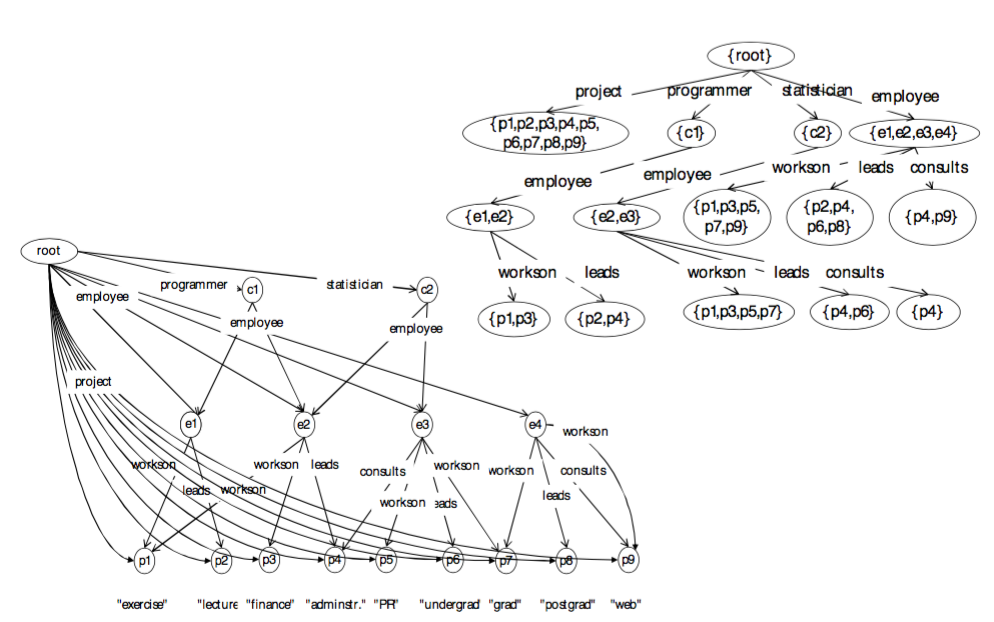
\includegraphics[width=\textwidth]{figures/data_guide.png}
\paragraph{Properties}
\begin{itemize}
\item Same nodes of data graph occur in multiple places $\rightarrow$ space complexity! Problem: node equivalence (if the paths leading to two nodes in the data graph are the same, the nodes are equivalent)
\item Repeating structures in the data graph are reduced to a single structure in the data guide (less edges)
\item Sometimes it can be more complex than the data graph itself
\item Deterministic graph = DFA. It is minimal, deterministic schema graph with 1:1  correspondence among data guide nodes and sets of nodes reached by the  same paths (strong dataguide)
\item Cycles in the data graph lead to cycles in the data guide
\end{itemize}

\paragraph{Semistructured Data Indexing}
As the data guide is deterministic we can use it as an indexing structure (each data guide node stores for each label the data guide node reached by the label and the graph database nodes). Answering a query is simple:
\begin{itemize}
\item for a non-terminal query element look-up the next data guide node
\item for a terminal element look-up the graph database nodes
\end{itemize}

\subsubsection{Language Equivalence}
To overcome the space complexity of data guides, non-deterministic schema graphs could be used. We can observe that if the set of paths leading to two nodes in the data graph are the same, the nodes are equivalent from the viewpoint of query processing. Formal definitions:
\begin{itemize}
\item Language: set of all possible paths to node x. L$_{x}$ = {p = p$_{1}$..p$_{n}$ p is a path from the root to x}
\item Language equivalent nodes: x $\equiv$ y if L$_{x}$ = L$_{y}$
\item Equivalence class of x denoted as [x]
\end{itemize}
Then we can create one node for language equivalent nodes. 
Drawback: checking for language equivalence is pspace complete. Solution: approximate language equivalence by a computationally more feasible relation. 

\paragraph{Approximation}A relation $\approx$ is an approximation of $\equiv$ if $\forall$ x,y: x $\approx$ y $\rightarrow$ x $\equiv$ y. 
\\
Queries will be correctly answered but query evaluation will be more expensive as there are more nodes to be checked. The reverse bisimulation is such a relationship. 

\paragraph{Reverse Bisimulation}
\begin{itemize}
\item It is equivalent to the simulation relation in both directions with the edges of the graphs inverted
\item On any graph there exists a maximal reversed bisimulation relation which can be efficiently computed and $\forall$ x,y: x $\approx$ y $\rightarrow$ x $\equiv$ y
\item If x $\approx$ y and x is the root then y is the root, and vice versa. If x $\approx$ y and there exists an edge x' $\rightarrow$$_{l}$ x then there exists an edge y' $\rightarrow$$_{l}$ y and x' $\approx$ y', and vice versa. 
\end{itemize}

\paragraph{Index Construction} 
\begin{itemize}
\item Every equivalence class is one node of the index graph. The nodes are connected with a labeled edge if such an edge exists between the members of the equivalence class in the data graph. 
\item This is an \textbf{unambiguous} definition since the equivalence classes cannot be distinguished from the viewpoint of accessibility through paths (either all members of two equivalence classes are connected by a labeled edge or none, otherwise the classes would be different).
\item Query processing will in general have to follow multiple paths in the non-deterministic data guide.
\item The index cannot be larger than the database itself.
\item The hash table for a node contains the key (label of outgoing edge), the corresponding index graph node and the data graph nodes for this index.
\end{itemize}

\subsection{Schema Mapping}
The goal is to integrate data that are available in two graph databases and that are semantically related to each other. So given two graph schemas S1 and S2 with two graph databases D1 and D2 we need to find a 1:1 matching of schema nodes (classes) that have the same or similar meaning (same or similar instances). Issue: D1 and D2 might have different extensions.

\subsubsection{Jaccard Similarity}
We can measure the level of similarity at the content level using the Jaccard Similarity. Let U be the finite set of possible instances, A and B classes which are subsets of U. 
\[
  sim(A,B) = \frac{|A \cap B|}{|A \cup B|} = \frac{P(x \in A \land x \in B)}{P(x \in A \lor x \in B} = \frac{P(A,B)}{(P(A,B)+P(\bar{A},B)+P(A,\bar{B}))}
\]
We can notice that if A has leaf nodes and the instances of B are complex data the similarity would be 0 even if B contains the same instances as A at the leaf level, that's why we introduce the features of classes.

\subsubsection{Features of Classes}
Content feature = set of terms associated with the paths of a node $i$ to the leaves with repeated occurrences $T_{i} = \{t_{1},...,t_{n}\}$, simply all the leaves from a node $i$.

\subsubsection{Probabilistic Approach: Naive Bayes Classifier}
Directly comparing the features does not always help to detect the correspondences as due to different database extensions and different naming conventions, even classes that have a strong semantic similarity often have no common instances in two different databases. We may assume that $U1 \cap U2 = \emptyset$.
\\
We cannot compute P(A,B) directly. A better approach would be: given $i \in B$ would be likely that also $i \in A$, even if $i$ is not part of U1. We can construct a function that gives the probability for a given instance $i$ with feature $T_{i}$ to belong to a class A, using Bayes law:
\[
  P(A|T_{i}) = P(T_{i}|A)P(A)
\]
This is the Na�ve Bayes Classifier.
\\
We know that:
\begin{itemize}
\item $P(A) = \frac{|A|}{|U_{1}|}$ 
\item $P(t_{i}|A) = P(t_{1}|A)...P(t_{n}|A)$, by independence assumption 
\item $P(t|A) = \frac{|t \in T_{A}|}{\sum_{t'}{|t' \in T_{A}|}}$ 
\end{itemize}

\subsubsection{Steps to compute similarity between classes A and B}
\begin{itemize}
\item take all instances of U1 and train a classifier to decide whether an instance belongs to A or not
\item take all instances in U2 and split into U2$^{B}$ and U2$^{\bar{B}}$
\item apply the classifier trained with U1 to all instances in U2 to produce sets U2$^{AB}$,  U2$^{A\bar{B}}$,  U2$^{\bar{A}B}$
\item do the same with the roles of U1 and U2 inverted
\item compute $P(A,B) = \frac{|U1_{AB}|+|U2_{AB}|}{|U1|+|U2|}$, same for $P(A, \bar{B})$, etc.
\item compute for each pair of concepts sim(A,B) using Jaccard Similarity.
\end{itemize}
Instead of taking instances as a whole, we can tokenize the instance's name and compute P(word|concept). 
\subsubsection{Node Mapping}
Having the similarity values, alternative class mappings are possible. A naive approach: first the best matches are used to produce mappings, then the mapped classes are removed (to assure that each class is mapped to a unique other class) and then the process continues.